\subsection{Generische key-based Routing API}
\label{chap:grundlagen:api}
Verschiedene Typen und Implementierungen von p2p-Netzwerken haben sehr unterschiedliche Schnittstellen zur Programmierung, obwohl die Anwendungsfälle meist gleicher Art sind. Dabek moniert diese unterschiedlichen Schnittstellen der verschiedenen strukturierten p2p-Netzwerke, die häufig anhand dem Prinzip des \ac{kbr} agieren \cite{Dabek2003Towards}. Dies mache es aus Entwicklersicht schwer, vom Netzwerk zu abstrahieren und dieses gegebenenfalls zu wechseln. Dabek untersucht verschiedene strukturierte p2p-Netzwerke und identifiziert ein minimales Set von Funktionen. Diese sind in zwei Zuständigkeitsbereiche aufgeteilt: \enquote{Routing messages} und \enquote{Routing state access}.\\
Erstere umfassen drei Methoden, von denen zwei \enquote{Upcalls} sind. Ein Upcall ist ein Callback der Applikation, die vom Netzwerk aufgerufen wird. \texttt{route} ermöglicht das Senden einer Nachricht. Dabei kann ein Hinweis an das Netzwerk übergeben werden, über welchen Knoten die Nachricht als nächstes geroutet werden soll. Der Upcall \texttt{forward} wird auf jedem Knoten aufgerufen, der eine Nachricht weiterleitet. Als Parameter werden der Schlüssel, die Nachricht und der nächste Routingknoten übergeben. Alle Parameter können verändert werden und der Nachrichtenversand kann auch terminiert werden. Auf dem eigentlichen Empfänger der Nachricht wird zusätzlich vor \texttt{upcall} noch \texttt{forward} aufgerufen. Als Parameter werden der Schlüssel und die Nachricht übergeben.\\
\Fref{fig:routing_kbr} verdeutlicht die Aufrufreihenfolge. Angenommen eine Nachricht an Knoten \texttt{0x7b} wird von Knoten \texttt{0x3f} über \texttt{0x4a} und \texttt{0x64} geroutet. An Knoten \texttt{0x3f} wird die Nachricht mittels \texttt{route} an das Netzwerk übergeben. Die Applikation wird an den Knoten \texttt{0x4a} und \texttt{0x64} durch den Callback \texttt{forward} über die Nachricht informiert. Am Zielknoten \texttt{0x7b} wird diese jedoch nicht direkt mittels \texttt{deliver} an die Applikation übergeben, sondern erst einer Bearbeitung durch \texttt{forward} zugeführt. Jeder Knoten kann in \texttt{forward} anhand des übergebenen nächsten Routingknotens feststellen, ob er der zuständige Knoten ist. Dadurch wird zum Beispiel dem Empfänger die Möglichkeit gegeben, die Nachricht zu verändern um diese bespielsweise an einen anderen Knoten weiterzuleiten.

\begin{figure}[htbp]
\centering
\resizebox{\textwidth}{!}{%
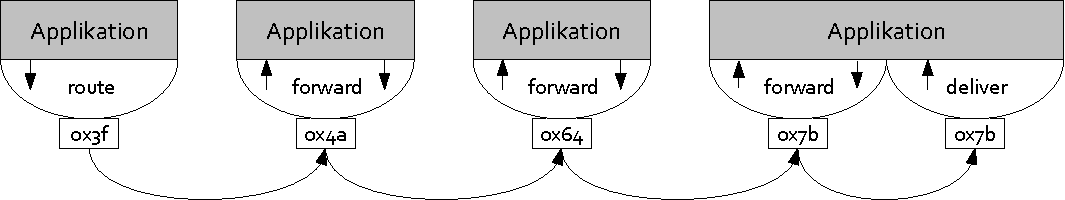
\includegraphics{grafics/routing_kbr.pdf}}
\caption{Routing einer Nachricht und Aufruf der Callbacks}
\label{fig:routing_kbr}
\end{figure}


\enquote{Routing state access} umfasst vier Methoden und einen Upcall. Dieser, \texttt{update}, informiert über Knoten, die das Netzwerk betreten oder es verlassen. Die Methode \texttt{local\_lookup} wird genutzt, um eine Liste möglicher Knoten, die als nächster Routinghop in Frage kommen, anzufragen. \texttt{neighborSet} liefert eine Liste der Nachbarn des aktuellen Knotens. Soll ein Datensatz auf mehreren Knoten gespeichert werden, ist die Methode \texttt{replicaSet} nützlich. Diese liefert für einen gegebenen Schlüssel eine Liste aller Knoten, die für den Datensatz geeignet sind. Um den Bereich zu ermitteln, für den der eigene Knoten zuständig ist, wird die Methode \texttt{range} angeboten.

Dabek zeigt, dass dieses \acf{api} ausreichend ist, um darauf aufbauend verschiedene Anwendungen wie Publish/Subscribe zu implementieren. Er beschreibt ebenfalls, wie einige Systeme -- namentlich CAN, Chord, Pastry und Tapestry -- an diese \ac{api} anzupassen sind.
